%
% Planteaminto del problema,
% presentación en RCI.
% Proyecto Lovelace.
%

\section{El problema de la protección de datos bancarios}

\begin{frame}{El problema de la protección de datos bancarios}
  \begin{itemize}
    \item El crecimiento del comercio en línea, aunado a sistemas débilmente
      protegidos, propició un incremento en los robos de datos bancarios.
  \end{itemize}
  \begin{figure}
    \centering
    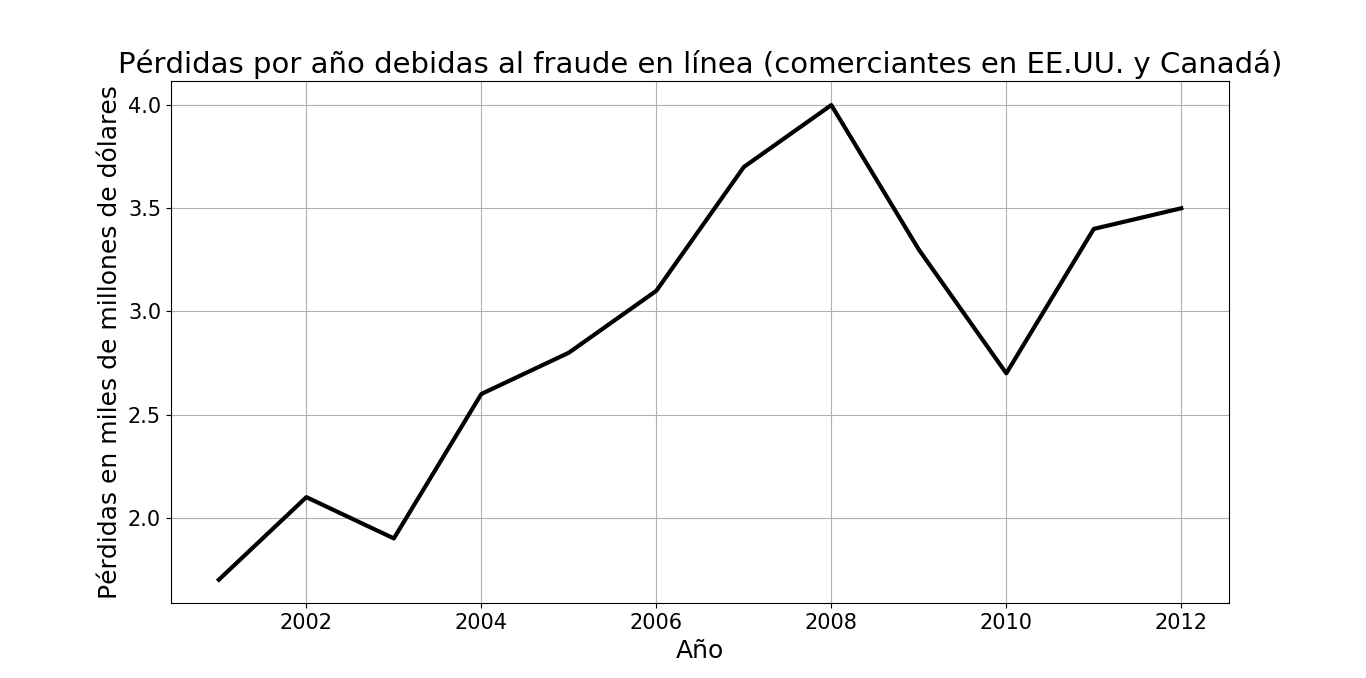
\includegraphics[width=0.85\linewidth]
       {diagramas_comunes/estadisticas_fraudes/perdidas_fraude_2002_2012.png}
    \caption{Pérdidas debidas al fraude en línea (2001-2012)~\cite{wallethub}.}
  \end{figure}
\end{frame}

\begin{frame}{El problema de la protección de datos bancarios}
  \begin{figure}
    \centering
    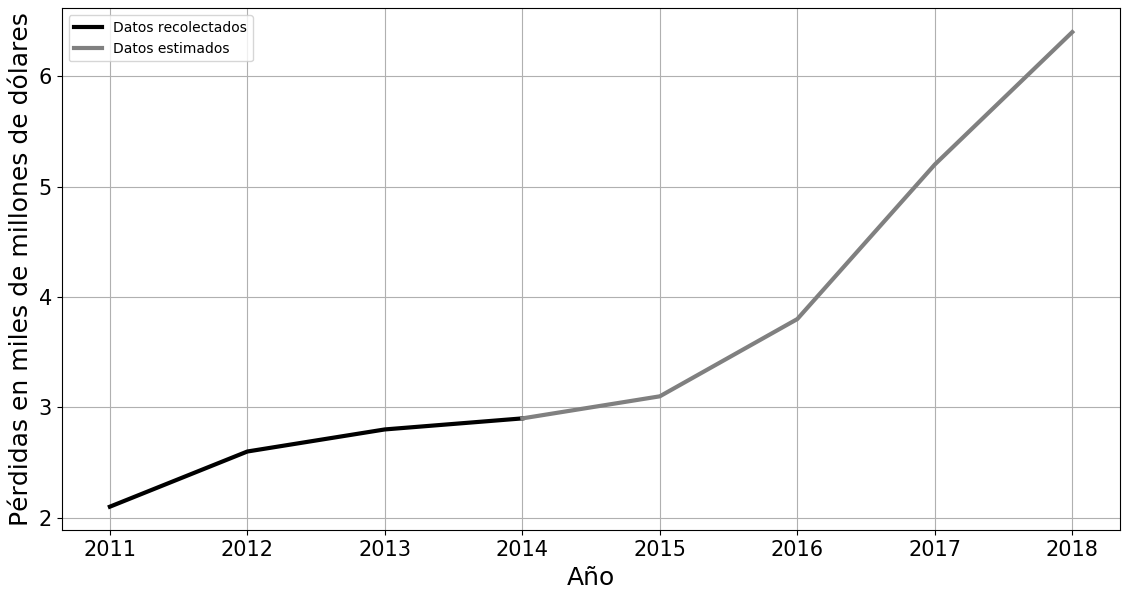
\includegraphics[width=1\linewidth]
       {diagramas_comunes/estadisticas_fraudes/perdidas_fraude_2011_2018.png}
    \caption{Pérdidas debidas al fraude con tarjetas no presentes (CNP) en
              EE.~UU. (2011-2018)~\cite{creditcards}.}
  \end{figure}
\end{frame}

\begin{frame}{El problema de la protección de datos bancarios}
  \begin{itemize}
    \item En el 2004 se publicó el PCI DSS\footnotemark \cite{pci_dss}.
    \item Hasta este momento el enfoque era proteger la información en donde
      sea que se encuentre.
    \item A pesar de la publicación del estándar, las filtraciones de datos
      no han cesado.
  \end{itemize}
  \footnotetext{\textit{Payment Card Industry, Data Security Standard}}
\end{frame}
